\documentclass{sig-alternative}
% \documentclass[conference]{IEEEtran}
\usepackage{color}
\usepackage{listings}
\usepackage{graphics} 
\usepackage{cite}
\usepackage{rotating}
\usepackage{eqparbox}
\usepackage{graphics}
\usepackage{colortbl} 
\usepackage{times}
\usepackage{balance}
\usepackage{picture}
\usepackage{algorithm}
\usepackage{algorithmicx}
\usepackage{algpseudocode}
\usepackage[export]{adjustbox}
\renewcommand{\footnotesize}{\scriptsize}
\definecolor{lightgray}{gray}{0.8}
\definecolor{darkgray}{gray}{0.6}
\renewcommand{\algorithmicrequire}{\textbf{Input:}}
\renewcommand{\algorithmicensure}{\textbf{Output:}}
\usepackage[table]{xcolor}
\definecolor{Gray}{rgb}{0.88,1,1}
\definecolor{Gray}{gray}{0.85}
\definecolor{Blue}{RGB}{0,29,193}
\newcommand{\G}{\cellcolor{green}}
\newcommand{\Y}{\cellcolor{yellow}}


\definecolor{MyDarkBlue}{rgb}{0,0.08,0.45} 
\lstset{
    language=Python,
    basicstyle=\ttfamily\fontsize{2.7mm}{0.8em}\selectfont,
    breaklines=true,
    prebreak=\raisebox{0ex}[0ex][0ex]{\ensuremath{\hookleftarrow}},
    frame=l,
    showtabs=false,
    showspaces=false,
    showstringspaces=false,
    keywordstyle=\bfseries,
    emph={furthest,gale,better,improved,where,fastmap,split,project,mutate,mutate1}, emphstyle=\bfseries\color{blue},
    stringstyle=\color{green!50!black},
    commentstyle=\color{gray}\itshape,
    numbers=left,
    captionpos=t,
    escapeinside={\%*}{*)}
}


%%% graph
\newcommand{\crule}[3][darkgray]{\textcolor{#1}{\rule{#2}{#3}}}
%\newcommand{\rone}{\crule{1mm}{1.95mm}}
%\newcommand{\rtwo}{\crule{1mm}{1.95mm}\hspace{0.3pt}\crule{1mm}{1.95mm}}
%\newcommand{\rthree}{\crule{1mm}{1.95mm}\hspace{0.3pt}\crule{1mm}{1.95mm}\hspace{0.3pt}\crule{1mm}{1.95mm}}
%\newcommand{\rfour}{\crule{1mm}{1.95mm}\hspace{0.3pt}\crule{1mm}{1.95mm}\hspace{0.3pt}\crule{1mm}{1.95mm}\hspace{0.3pt}\crule{1mm}{1.95mm}} 
%\newcommand{\rfive}{\crule{1mm}{1.95mm}\hspace{0.3pt}\crule{1mm}{1.95mm}\hspace{0.3pt}\crule{1mm}{1.95mm}\hspace{0.3pt}\crule{1mm}{1.95mm}}
\newcommand{\quart}[3]{\begin{picture}(100,6)%1
{\color{black}\put(#3,3){\circle*{4}}\put(#1,3){\line(1,0){#2}}}\end{picture}}
\definecolor{Gray}{gray}{0.95}
\definecolor{LightGray}{gray}{0.975}
% \newcommand{\rone}{}
% \newcommand{\rtwo}{}
% \newcommand{\rthree}{}
% \newcommand{\rfour}{} 
% \newcommand{\rfive}{}
\newcommand{\wei}[1]{\textcolor{red}{Wei: #1}} 
\newcommand{\Menzies}[1]{\textcolor{red}{Dr.Menzies: #1}} 

%% timm tricks
\newcommand{\bi}{\begin{itemize}[leftmargin=0.4cm]}
\newcommand{\ei}{\end{itemize}}
\newcommand{\be}{\begin{enumerate}}
\newcommand{\ee}{\end{enumerate}}
\newcommand{\tion}[1]{\S\ref{sect:#1}}
\newcommand{\fig}[1]{Figure~\ref{fig:#1}}
\newcommand{\tab}[1]{Table ~\ref{tab:#1}}
\newcommand{\eq}[1]{Equation~\ref{eq:#1}}

%% space saving measures

\usepackage[shortlabels]{enumitem}  
\usepackage{url}
% \def\baselinestretch{1}


% \setlist{nosep}
%  \usepackage[font={small}]{caption, subfig}
% \setlength{\abovecaptionskip}{1ex}
%  \setlength{\belowcaptionskip}{1ex}

%  \setlength{\floatsep}{1ex}
%  \setlength{\textfloatsep}{1ex}
%  \newcommand{\subparagraph}{}

% \usepackage[compact,small]{titlesec}
% \DeclareMathSizes{7}{7}{7}{7} 
% \setlength{\columnsep}{7mm}

\begin{document}
% \conferenceinfo{FSE}{'15 Bergamo, Italy}
\title{ Performance Modelling: Clustering meets Sampling}
\numberofauthors{2}
\author{
        \alignauthor Vivek Nair, Tim Menzies, Xipeng Shen 
        \affaddr{Computer Science, North Carolina State University, Raleigh, USA}
        \email{vivekaxl, tim.menzies, xipengshen@gmail.com}
    \and  
        \alignauthor Norbert Siegmund, Sven Apel \\
        \affaddr{Computer Science, University of Passau, Germany}\\
        \email{norbert.siegmund, apel@uni-passau.de}
       }

\maketitle 
\thispagestyle{plain}
\pagestyle{plain}
\begin{abstract}
Active Learning, Configuration, Sampling, Machine Learning, Performance Prediction


\end{abstract}

% A category with the (minimum) three required fields
\vspace{1mm}
\noindent
{\bf Categories/Subject Descriptors:} 
D.2 [Software Engineering] ;
I.2.6 [Artificial Intelligence]: Induction

 
\vspace{1mm}
\noindent
{\bf Keywords:} Performance prediction, Active Learning, 
Multi-Objective Optimization,
Search-based Software Engineering,Sampling, Machine Learning.

\pagenumbering{arabic} %XXX delete before submission
 
 
\section{Introduction}
 
\bi
    \item{Challenges}
    \item{Solutions Proposed}
    \item{Research Questions}
\ei
\section{Bird's Eye Overview}
\bi
    \item{Sampling}
    \item{Fast Learners}
\ei

\section{Problem Formulation}

\bi
    \item{Tables}
    \item{Feature Models}
    Feature Model(FM) defines all the N features and all the valid configurations C of a software system. Figure \textcolor{red}{(add figure)} shows the feature model of Berkeley DB(C Version) using the notations defined in ~\cite{kang1990feature}, ~\cite{guo2012consistency}. Feature models are used to check the validity of new mutated solutions generated by the learners (eg. GALE).
    
\begin{figure}[!t]
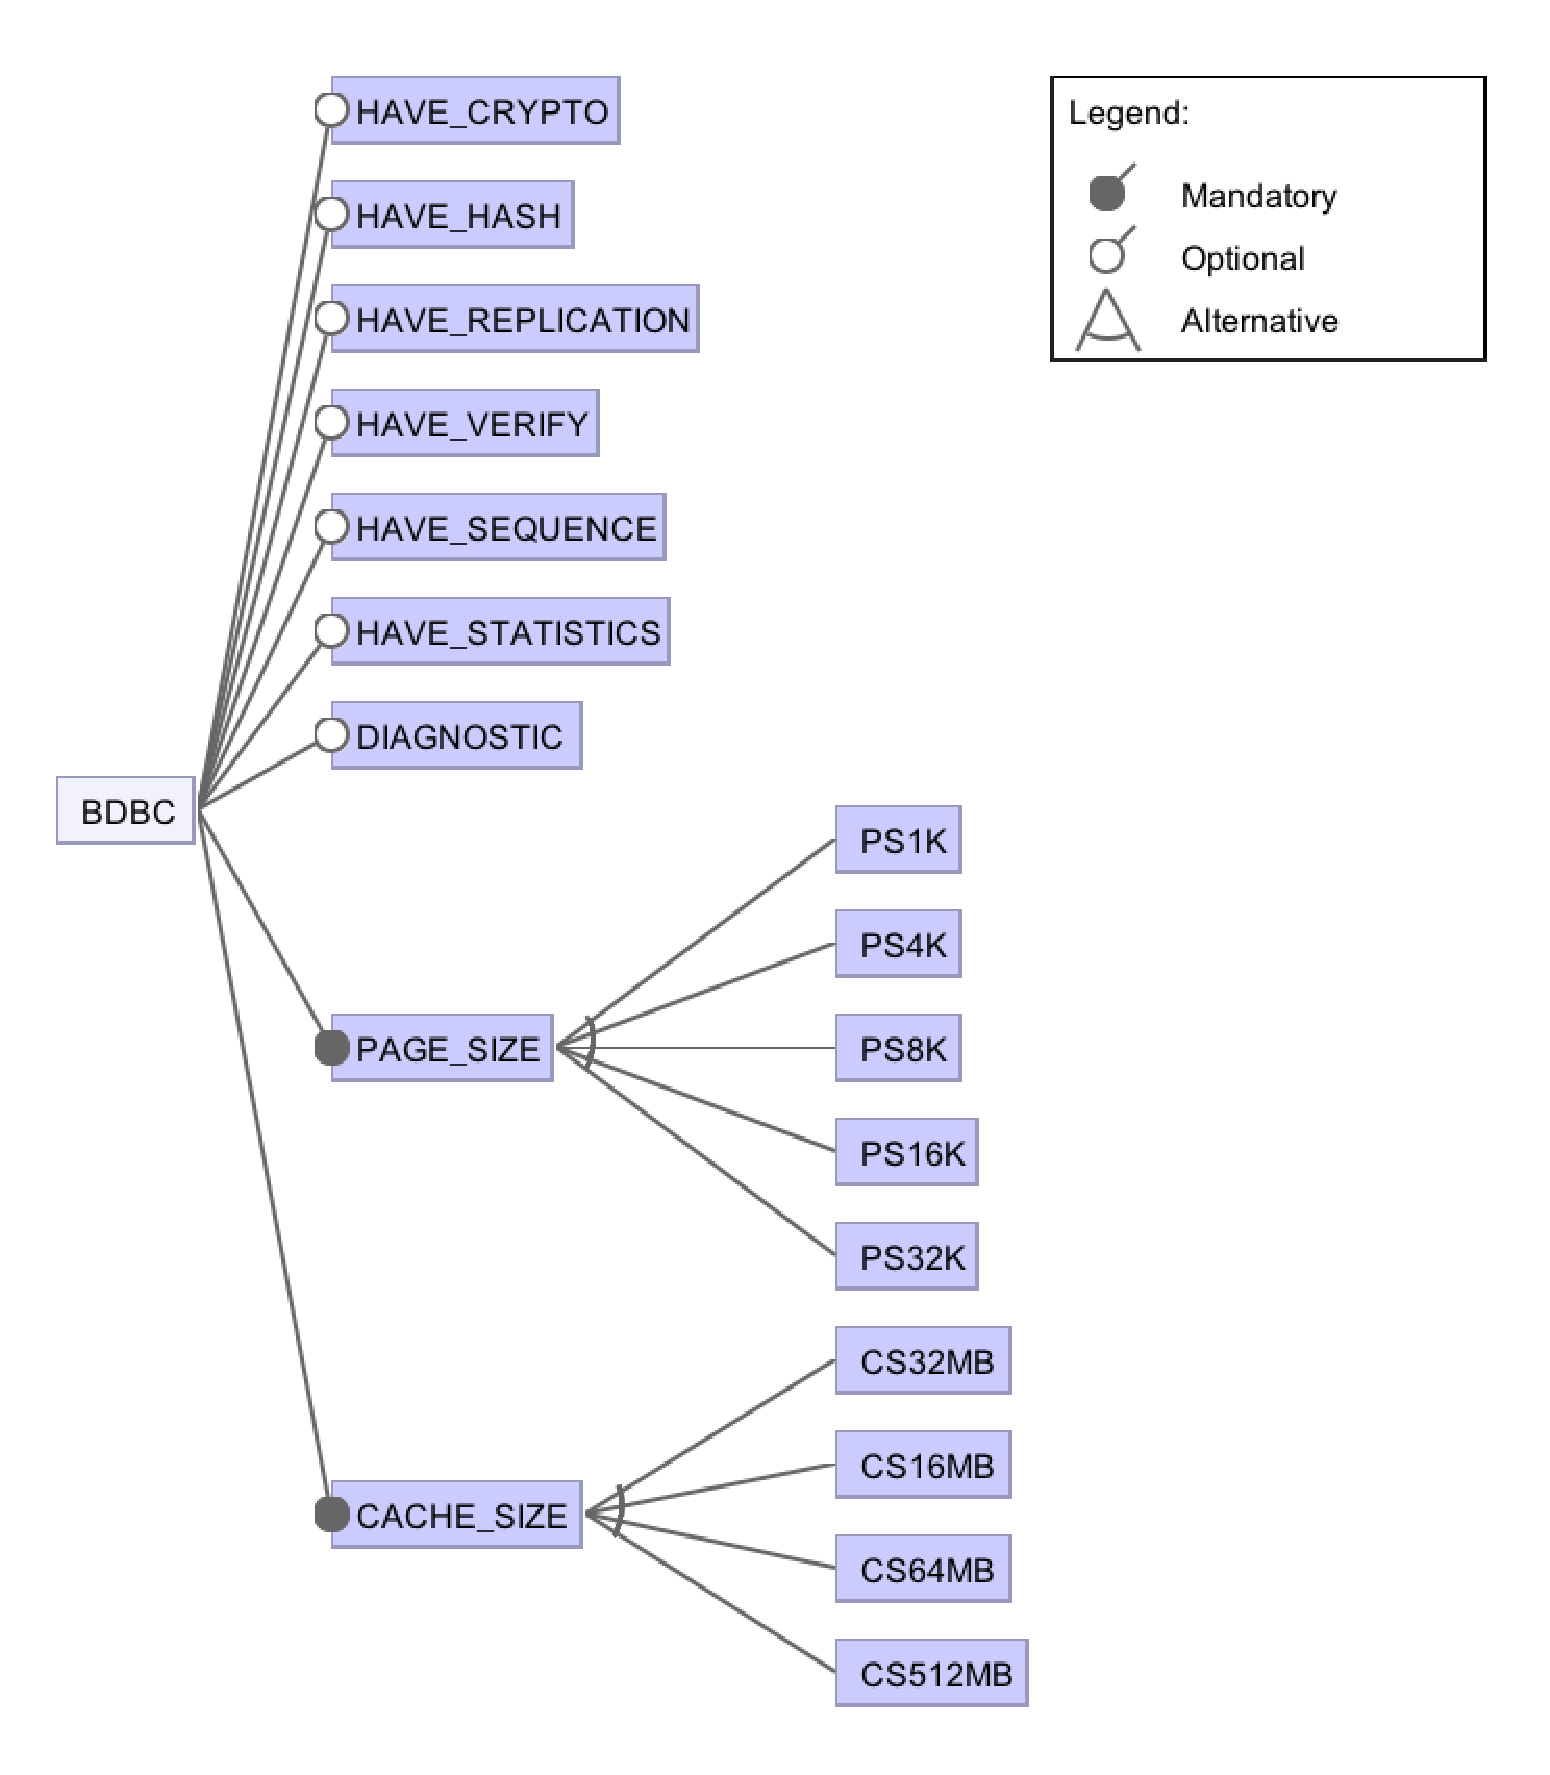
\includegraphics[width=0.9\linewidth]{Figures/BDBC.eps}
\caption{ Berkeley database feature model   (``C'' version). }\label{fig:bdbc}
\end{figure}
    
    \item{Data Definition}
    The features on the software system is represented as a set of binary decision variables. A feature, when turned on, corresponds to 1, and 0 otherwise. All the features of a system is represented a vector F = $<f_1, f_2, ...,f_N>$, where N is the number of features of the software system. The dependent variable corresponding to a configuration(F) is a performance score, P(F), which the performance measurement.
    \item{Learning Problem}
    Performance of system can be modelled using the configuration as the independent variable and the performance metric as a dependent variable. Modelling a software system is to find a hypothesis function(h), such that h(F) predicts P(F) accurately. This can be represented as:\\
\begin{center}
    $ h: C \mapsto \rm I\!R$ s.t. $L(h(F), P(F))$ is minimized\\
\end{center}

where, L is a loss function for penalizing errors in prediction. By formulating the performance prediction using the method described, we can transform the problem into a learning problem. 
    It should be noted that though the number of possible configurations (C) is equal to $2^N$(binary decision variables), in reality valid configurations(\^{C}) is smaller than C (|C| << |\^C|). 
    
\ei

 \begin{figure}[!t]
\scriptsize
\begin{tabular}{llllll}
  \hline
Project & Domain & Lang. & LOC & Features & Config\\\hline
BDBC: Berkeley DB   & Database & C & 219,811 & 18 & 2560\\
BDBJ: Berkeley DB   & Database & Java & 42,596 & 32  & 400\\
Apache & Web Server & C & 230,277 & 9 & 192\\
SQLite & Database & C & 312,625 & 39 & 3,932,160\\
LLVM & Compiler & C++ & 47,549 & 11 & 1024\\
x264 & Video Enc. & C& 45,743 & 16 & 1152\\\hline
\end{tabular}
 
\caption{Siegmund data.
For SQLite, the data  contains 4,553 configurations for prediction modeling and 100 additional random configurations for prediction evaluation, see \cite{vapp}.}\label{fig:cpm}
\end{figure}


 \begin{table}[!t]
 

 \begin{tabular}{c c } 
 \hline
 Project & Benchmark/Job Used  \\  
 \hline
 Berkeley DB CE & Vendor Provided  \\ 
 
 Berkeley DB JE & Vendor Provided \\

 Apache & autobench + httperf \\

 SQLite & Vendor Provided \\
 
 LLVM & opt-tools \\ 

 x264 & Sintel(735MB) \\
 

\label{BenchMarkUsed} 
\end{tabular}
\caption{Overview of the benchmarks used in the evaluations}
\end{table}
\section{Sampling Technique: East-West Where}

\subsection{Approach}
\bi
    \item{WHERE}
\ei
\subsection{WHERE Learning}\label{sec:spectral}
This section describes how a large space of candidate solutions (configurations) into many smaller regions.

WHERE is a {\em spectral learner}~\cite{kamvar2003spectral}; i.e. given solutions with $d$ possible decisions(features), it re-expresses those $d$ decision variables in terms of the $e$ eigenvectors of that data.
This speeds up the reasoning since we then only need to explore the $e\ll d$   eigenvectors.

A widely-used spectral learner is a principal components analysis (PCA). For example, PDDP ({\em Principal Direction Divisive Partitioning})~\cite{boley1998principal} recursively partitions data according to the median point of data projected onto the first PCA component of the current partition.

WHERE~\cite{me12d} is a linear time variant of PDDP  that uses FastMap~\cite{Faloutsos1995} to quickly find the first component.
Platt~\cite{platt05} shows that FastMap is a  Nystr\"om algorithm that finds approximations to eigenvectors.
As shown in \fig{fastmapCode} on lines 3,4,5, FastMap  projects all data onto a line connecting two distant points\footnote{
To define distance, WHERE uses the standard Euclidean distance method proposed by Aha et al.~\cite{aha91}; that is: $dist(x,y)= \sqrt{\sum_{i\in d} (x_i - y_i)^2}/\sqrt{ \left\vert{d}\right\vert }$ where distance is computed on the independent decisions $d$ of each candidate solution; all $d_i$ values are normalized min..max, 0..1; and the calculated distance normalized by dividing by the maximum distance across the $d$ decisions.}. 
FastMap finds these two distant points in near-linear time. 
The search for the poles needs only $O(N)$ distance comparisons (lines 19 to 24).
The slowest part of this search is the sort used to find the median $x$ value (line 10) but even that can be reduced to  asymptotically optimal linear-time via the standard median-selection algorithm~\cite{hoare61}.

FastMap returns the data split into two equal halves.
WHERE recurses on the two halves, terminating when some split has less than $\sqrt{N}$ items.


\begin{figure}[!t] 
\begin{minipage}{3.2in}
\begin{lstlisting}[mathescape,frame=l,numbers=left]
def fastmap(data): 
  "Project data on a line to 2 distant points"
  z          = random.choose(data)
  east       = furthest(z, data)
  west       = furthest(east, data)
  data.poles = (west,east)
  c          = dist(west,east)     
  for one in data.members: 
    one.pos = project(west,east,c,one)
  data = sorted(data) # sorted by 'pos'
  return split(data)

def project(west, east, c, x): 
  "Project x onto line east to west"
  a = dist(x,west)
  b = dist(x,east)
  return (a*a + c*c - b*b)/(2*c) # cosine rule

def furthest(x,data): # what is furthest from x?
  out, max = x,0
  for y in data:
    d = dist(x,y)
    if d > max: out, max = y, d
  return out

def split(data): # Split at median
   mid = len(data)/2; 
  return data[mid:], data[:mid]
\end{lstlisting}
\caption{Splitting data with FastMap}
\label{fig:fastmapCode}  
\end{minipage}
\end{figure}

We build the predictive model using the popular machine learning technique called Classification and Regression Tree(CART), which has been extensively used in the literature and has been observed to be fast and accurate~\cite{guo2013variability}.

\subsection{Results}
\begin{figure}[!t]
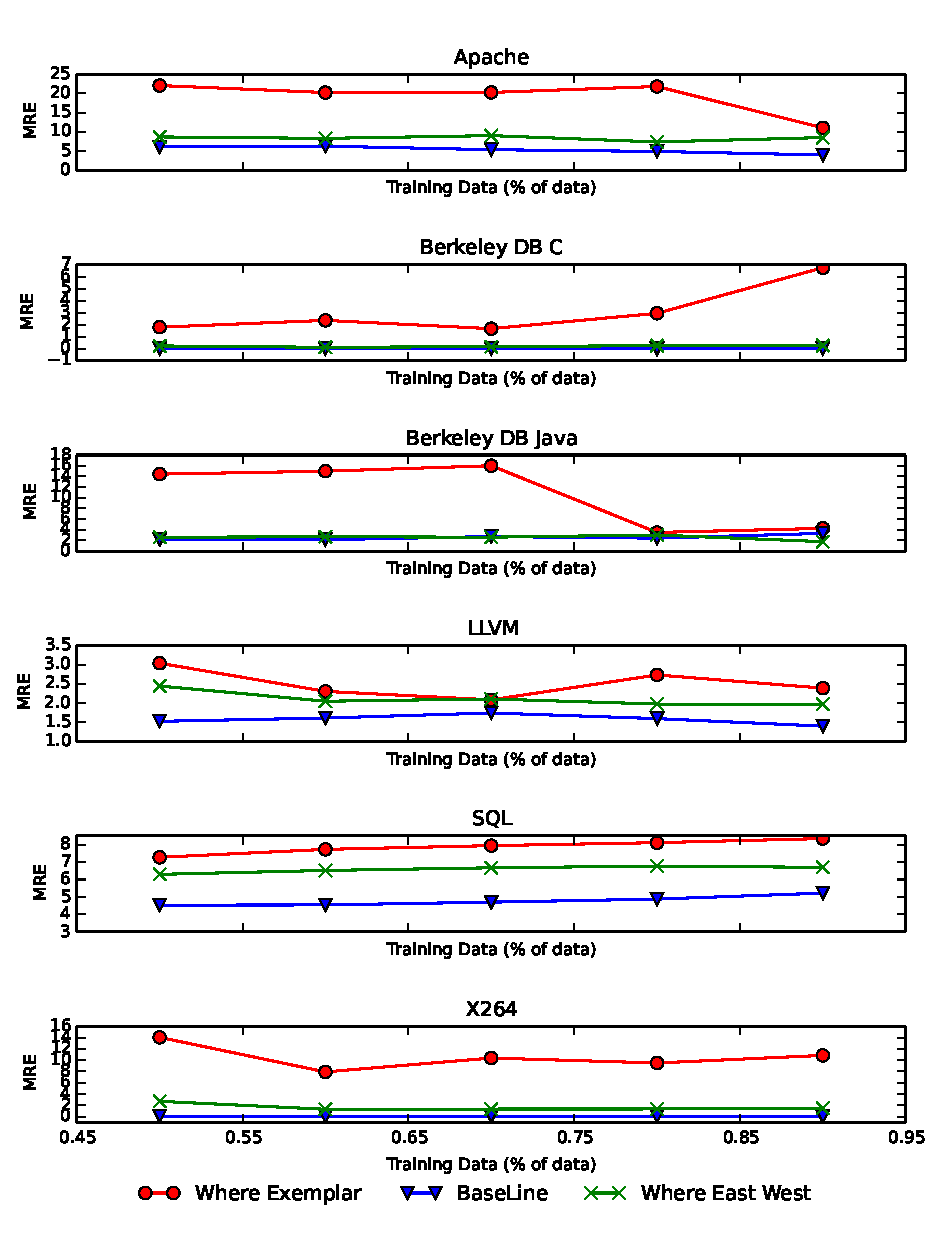
\includegraphics[width=0.9\linewidth]{Figures/SamplingAccuracy.eps}
\caption{Behavior of accuracy of WHERE-exemplar, baseline, WHERE-east-west wrt. to different training set sizes }\label{fig:sampling_accuracy}
\end{figure}

\begin{figure}[!t]
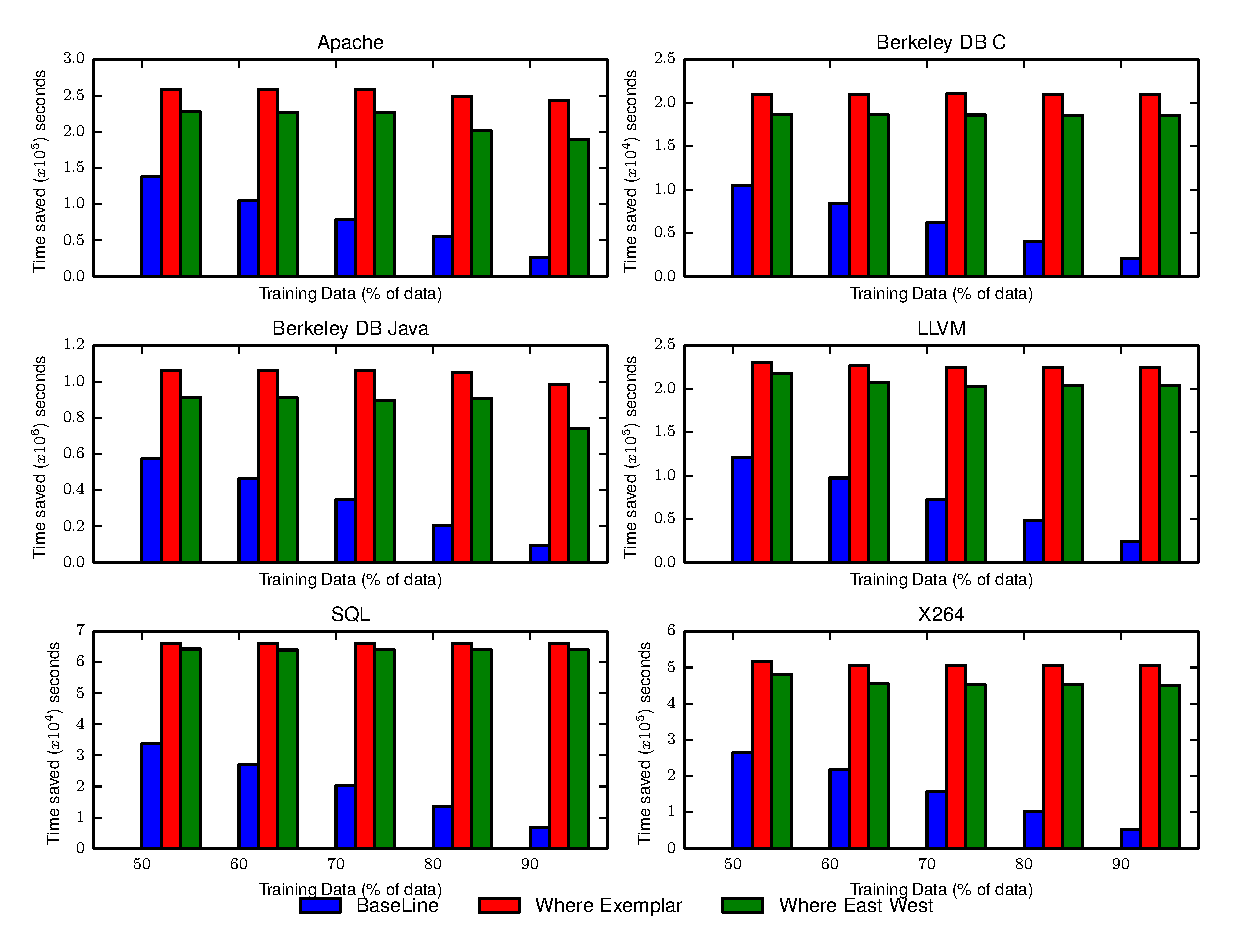
\includegraphics[width=0.9\linewidth]{Figures/performance_graph.eps}
\caption{Time saved by WHERE based techniques compared to the baseline techniques }\label{fig:performance_graph}
\end{figure}

\section{Fast Searcher: GALE}
\subsection{Approach}
\begin{figure}[!b]
\small
\begin{tabular}{|p{.95\linewidth}|}\hline
GALE initially builds a population of points by selecting decisions at random. It then {\em clusters} those decisions into neighborhoods as follows:
\begin{enumerate}
\item Find two distant points in that population; call them the {\em east} and {\em west} poles. 
\item Draw an axis of length $c$ between the poles. 
\item Let each point be at distance $a,b$ to the {\em east,west} poles.  Using the cosine rule, project each point onto the  axis  at $x=(a^2 + c^2 - b^2)/(2c)$.  
\item Using the median $x$ value, divide the population.
\item For each half that is larger than $\sqrt{N}$ of the original population, go to step 1.
\end{enumerate}

Note that the above requires a distance measure between sets of decisions: GALE uses the standard case-based reasoning measure defined by Aha et al.~\cite{aha91}. Note also that GALE implements step1 via  the FASTMAP~\cite{Faloutsos1995} linear-time
heuristic:
\begin{itemize}
\item Pick any point at random; 
\item Let {\em east} be the point furthest from that point; 
\item Let {\em west} be the point furthest from {\em east}.
\end{itemize}

These final sub-divisions found by this process are the {\em neighborhoods} that GALE will {\em perturb} as follows:
\begin{itemize}
\item Find the objective scores of the {\em east,west} poles in each neighborhood.
\item Using the continuous domination predicate of \fig{moea}, find  the {\em better} pole. 
\item Perturb all points in that neighborhood by pushing them towards the better pole, by a distance  $c/2$ (recall that  $c$ is the distance between the poles).
\item Let generation $i+1$ be the combination of all pushed points from all neighborhoods.
\end{itemize}

From a formal perspective, GALE is an active learner~\cite{Dasgupta2005} that builds a piecewise linear approximation to the Pareto frontier~\cite{Zuluaga:13}.  For each piece, it then pushes the neighborhood up the local gradient.  This  approximation is built in the reduced dimensional space found the FASTMAP  Nystr\"om approximation to the first component of PCA~\cite{platt05}.
\\\hline
\end{tabular}
\caption{Inside GALE}\label{fig:gale}
\end{figure}
GALE combines (a) the neighborhood perturbation (described above)  with (b)~the MOEA algorithm of \fig{moea}.  The algorithm reflects over a {\em population} of points, each of which contains {\em decisions} (some inputs to the CDA model).  It then searches for the input decisions that lead to best outcomes.  For example:
\begin{itemize}
\item if we adjust the inputs to model (say) high tailwind conditions\ldots
\item \ldots then GALE can report the best monitoring policies for the pilot of the cockpit instrumentation.
\end{itemize}

\fig{gale} lists the procedure by which GALE clusters the data into neighborhoods, then perturbs each neighborhood.  In terms of monitoring for brittleness, the key point of GALE is that this process continues until the perturbations stop having any new effect (i.e. they stop generating better objective scores). That is, all GALE solutions are guaranteed not to be brittle.


In terms of reducing runtime, the key feature of GALE is that unlike traditional MOEA methods such as NSGA-II~\cite{deb00afast}, GALE  does not automatically generate objective scores for all $N$ decisions.  Instead, as it recursively clusters the data in two (using steps 1,2,3,4,5 in \fig{gale}), GALE only computes the objective scores for the two most distant points in each division.  This means that this binary division of the data terminates after a comparison of just $log_2(N)$ evaluated individuals. This is much less than the $2N$ comparisons required by  traditional methods like NSGA-II.

In practice, this makes GALE run much faster than traditional optimization tools.  Standard MOEA algorithms such as NSGA-II require 3000 to 5000 evaluations to explore the CDA model. GALE, on the other hand, performs the same task using 25 to 50 evaluations~\cite{krallphd}. 

GALE's faster runtimes have  tremendous practical implications:
\bi
\item When checking for the stability of the conclusions reached from a randomizing
algorithm  such as GALE or NSGA-II, it is important to check that the conclusions hold in multiple repeats (say, 20 repeats). 
\item This number of repeats may practical for GALE but  highly impractical for standard optimization tools.
\item For example, twenty repeats of CDA takes 1.5 and 100 hours for GALE and NSGA-II, respectively~\cite{krallphd}.
\ei
\subsection{Results}

\begin{figure}[!t]
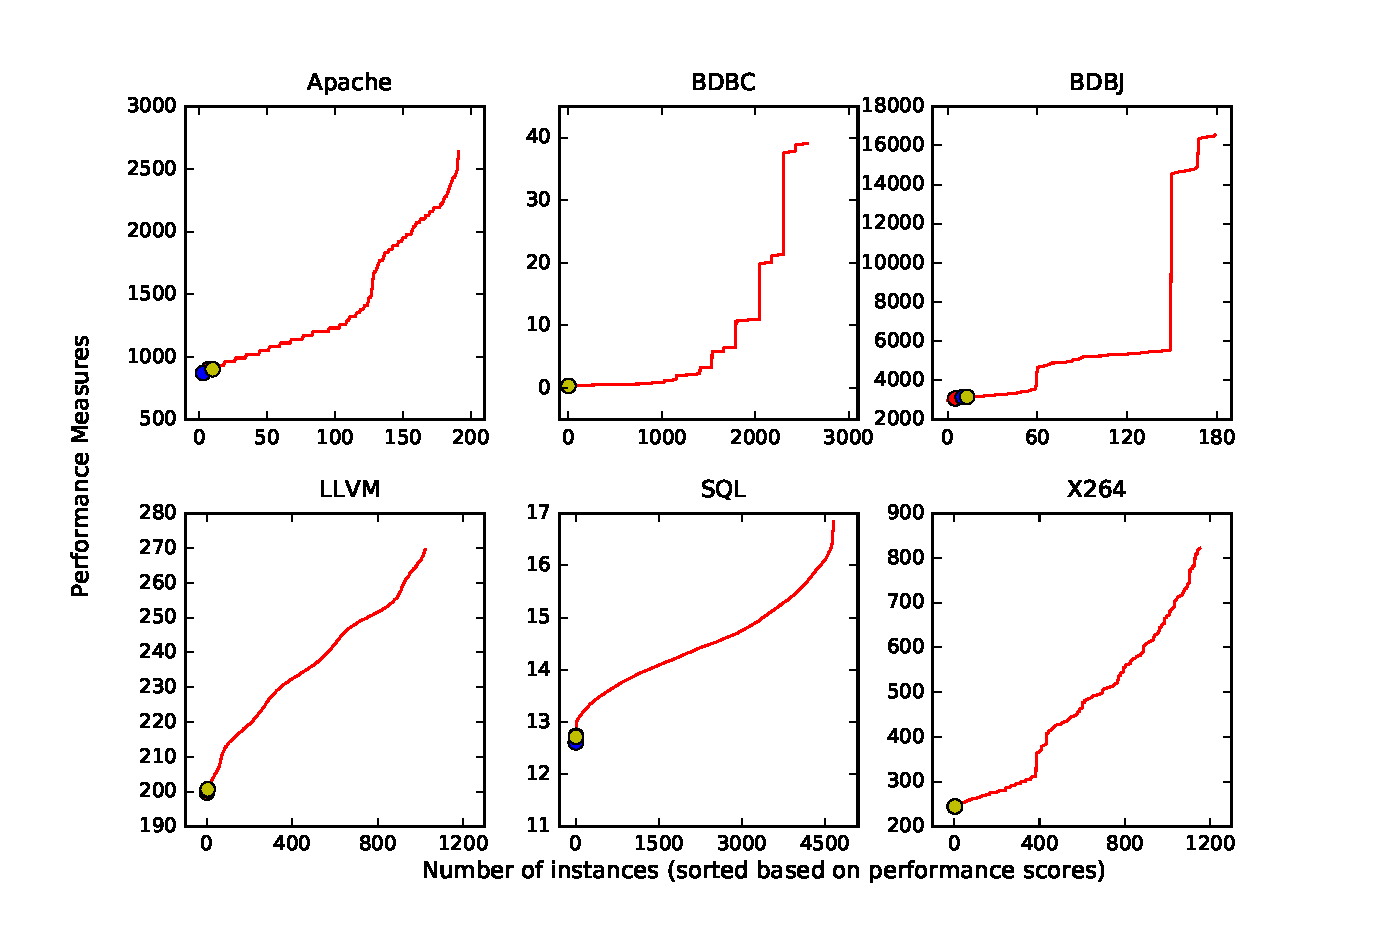
\includegraphics[width=0.9\linewidth]{Figures/optimizer_result.eps}
\caption{Solutions found by GALE}\label{fig:performance_graph}
\end{figure}


 
 
\section{Reliability and Validity}\label{sect:construct}


{\em Reliability} refers to the consistency of the results obtained
from the research.  For example,   how well independent researchers
could reproduce the study? To increase external
reliability, this paper has taken care to either  clearly define our
algorithms or use implementations from the public domain
(SciKitLearn). Also, all the data used in this work is available
on-line in the PROMISE code repository and all our algorithms
are on-line at github.com/ai-se/where.


{\em Validity} refers to the extent to which a piece of research actually
investigates what the researcher purports to investigate.
{\em Internal validity} checks if the differences found in
the treatments can be ascribed to the treatments under study. 
One internal validity issue with our experiments is the choice
of {\em training, tuning, and testing} data sets discussed in 
\tion{design}. Recall that while all our learners used the same
{\em testing} data set, our untuned learners were only given
access to {\em training} while DEs could get feedback from
{\em training} and
{\em tuning}.  This means that, potentially,  the performance increases
reported above are merely an artificat of the DEs being able to access
more data. However:
\bi
\item Note that
DEs assess their performance using a model built from {\em training}
then applied to the {\em tuning} data. If we gave the untuned
learners double the training data, then this would be inherently
biased against DEs.
\item In practice, this is much ado about nothing. We have
repeated all the experiments of this paper with the untuned
learners building models from {\em training} + {\em tuning}.
While the exact numbers found in this way
may differ from the above in some small way, we can report that 
those repeated runs do not substantively change the above conclusions.
\ei

{\em Internal validity}\textcolor{red}{(copied verbatim)}
Regarding SQLite, we cannot measure all possible configurations in reasonable time. Hence, we sampled only 100 configurations to compare prediction and actual performance values. We are aware that this evaluation leaves room for outliers.
Also, we are aware that measurement bias can cause false interpretations [20]. Since we aim at predicting performance for a special workload, we do not have to vary benchmarks.



{\em External validity} \textcolor{red}{(copied verbatim)} We aimed at increasing external validity by choosing programs from different domains with different configuration mechanisms and implemented with different programming languages. Furthermore, we used programs that are deployed and used in the real-world. Nevertheless, we are aware that the results of our evaluations are not automatically transferable to all configurable programs. In addition to our sample program selection, the strong and exhaustive evaluation (over 60 days of measurement with 5 computers) indicate that our heuristics hold for many practical application scenarios.

{\em Optimizer Bias} \textcolor{red}{(copied verbatim)}
Our reading of the literature is that the experimentation
in this paper is far larger than what is typically used
to certify new optimizers. Also, we know of no other
search-based SE paper that can achieve GALE’s results
using so few evaluations.
That said, the applicability of GALE to new models
is an open question. We have shown that GALE does
better than NSGA-II and DE, for the configuration search spaces explored
above. This is not to say that we we have not shown that
it works better than all optimizers over all data sets.
There are theoretical reasons to conclude that it is impossible
to show that any one optimizer always performs
best. Wolpert and Macready [NFL paper] showed in 1997 that no
optimizers necessarily work better than any other for all possible optimization problems.

{\em Parameter Bias} \textcolor{red}{(copied verbatim)}
For this study, we did not do extensive parameter tuning:
NSGA-II and DE were run using their default
settings while GALE was run using the settings that
worked well on the first model we studied, which were
then frozen for the rest of this study. As documented
above, those parameters were:
\begin{itemize}
\item $\mu$ = 100: population size;
\item $\omega$ = $\mu$: minimum size leaf clusters;
\item $\lambda$ = 3: premature stopping criteria (sets the maximum
allowed generations without any improvement
on any objective).
\item $\delta$ = 1: the ``accelerator'' that encourages larger
mutations;
\item $\gamma$ = 1.5: the ``brake'' that blocks excessive mutation.
\end{itemize}

If this paper was arguing that these parameters were
somehow optimal, then it would be required to present
experiments defending the above settings. However, our
claim is less than that—we only aim to show that with
these settings, GALE does as well than standard MOEA
tools. In future work, we will explore other settings.




That said, there exist some class of data mining papers for which
tuning may not be required. Consider  Le Goues et al.'s 2012
ICSE paper that used a evolutionary program to learn
repairs to code~
in that paper was ``can we fix any of the known bugs?''. Note
that this criteria is a ``{\em competency}'' statement, and
not a ``{\em better than}'' statement (the difference being that
one is 
``can do'' and the other is ``can do better''). For such
competency claims, tuning is not necessary. However, as soon
as {\em better than} enters the performance criteria then this
becomes a race between competing methods. In such a race,
it is unfair to hobble one competitor with poor tunings.



\section{Conclusions}

Our exploration of the six research
questions listed in the introduction
show that when learning defect predictors for static code
attributes,   analytics without parameter tuning is considered {\em harmful} and {\em misleading}:
\bi
\item Tuning improves the performance scores of a predictor.
That improvement is usually positive (see \fig{deltas}) and sometimes
it can be quite   dramatic (e.g. precision changing from 2\% to 98\%). \item 
Tuning changes conclusions on what learners are better than others.
Hence, it is time to revisit numerous prior publications of our own~
and others~
\item
Also,
tuning changes conclusions on what factors are most important in software development.
Once again, this means that old papers may need to be revised including those
some of our own~
\ei
Accordingly, we strongly advise that data miners should not be used ``off-the-shelf'' with their default tunings. 
\fig{features} shows just how much tuning can alter default settings
both for different data sets and for different goals. 

Since the results from tuning are unstable,
tuning needs to be repeated
whenever data or goals are changed.
Fortunately, the cost of find good tunings is not excessive since, at least for
static code defect predictors, tuning is easy and fast.

\section{Future Work}

 As noted by
F\"{u}rnkranz~
problem that seeks the smallest model with the highest performance, 
that generalizes best for
future examples (perhaps learned in minimal time using the least amount of data).
In this view, we are using DE to optimize an optimizer. Perhaps a better approach might be
to dispense with the separation of ``optimizer'' and ``learner'' and combine them both
into one system that learns how to tune itself as it executes. If this view is useful,
then instead of adding elaborations to data miners (as done in this paper, or by researchers
exploring hyper-heuristics~
mining with a single system that rapidly performs both tasks.

Another issue for future work is the implications of these
conclusions to other kinds of software analytics.
 This paper has explored  {\em some} learners using {\em one}  optimizer. Hence, we can make
no claim that DE is the {\em best} optimizer for {\em all} learners.
Rather, our point is that there exists at least some learners
whose performance can be dramatically improved by 
at least one simple optimization scheme.  We hope that this work inspires
much future work as this community develops and debugs best practices for tuning
software analytics.
 
 

\section*{Acknowledgments}
The work has partially funded by a National Science Foundation CISE CCF award \#1506586.
 
\vspace*{0.5mm}
 
 
\bibliographystyle{plain}

\balance
\bibliography{activeconfig}  

   



  


  

\end{document}
 
\subsection{Implications}

time for an end to era of data mining in se? moving on to a new phase of learning-as-optimization

1) learning is actually an optimization tasks (e.g. see fig2 of  learners climbing the roc curve hill in http://goo.gl/x2EaAm)

2) our learners are all contorted to do some tasks X (e.g. minimize expected value of entropy), then we assess them on score Y (recall). which is nuts. maybe we should build the goal predicate into the learner (e.g http://menzies.us/pdf/10which.pdf) 

3) given 1 + 2, maybe the whole paradigm of optimizing param selection is wrong. maybe what we need is a library of bees buzzing around making random choices (e.g. about descritziation) which other bees use, plus their own random choices (e.g. max depth of tree learned from discretized data) which is used by other bees, plus their own random choices (e.g. business users reading the models).  the funky thing here is that it can take some time before some of the bees (the discretizers) get feedback from the community of people using their decision (the tree learners). 




